\documentclass[conference]{IEEEtran}
\IEEEoverridecommandlockouts

% Notes for the authors (not printed):
% - Every number in this paper comes from the runs saved in results/ (final run: results/summary.md).
% - Citations that could not be verified were removed from the original draft:
%   "LoCoMo-Plus" (arXiv:2602.10715), "Cognitive AI Labs" (arXiv:2607.24368),
%   "Stateful SWE-bench" and the "Memori Labs" report. Re-add them only with a working link.
% - Multi-Session Chat is by Xu et al. (2022), not Zheng et al.

\usepackage{cite}
\usepackage{amsmath,amssymb,amsfonts}
\usepackage{graphicx}
\usepackage{textcomp}
\usepackage{xcolor}
\usepackage{booktabs}
\usepackage{array}
\usepackage{tikz}
\usetikzlibrary{arrows.meta,positioning}

% Allow long monospace identifiers to break instead of overflowing
\newcommand{\code}[1]{\texttt{\hyphenchar\font=45\relax #1}}
\newcommand{\cmark}{$\checkmark$}
\newcommand{\xmark}{$\times$}
% Left-aligned paragraph column for narrow table cells
\newcolumntype{L}[1]{>{\raggedright\arraybackslash}p{#1}}
% Slightly more tolerant line breaking in narrow columns
\emergencystretch=1.5em

\begin{document}

\title{ESD-Lite: Non-Destructive, Budget-Bounded Conversational Memory via Bi-Temporal Knowledge Graphs}

\author{\IEEEauthorblockN{Naeem Abdullah Sadik}
\IEEEauthorblockA{\textit{Department of Computer Science and Engineering}\\
\textit{United International University}\\
nsadik222115@bscse.uiu.ac.bd}
\and
\IEEEauthorblockN{Farhan Al Imam Somuddro}
\IEEEauthorblockA{\textit{Department of Computer Science and Engineering}\\
\textit{United International University}\\
fsomuddro222022@bscse.uiu.ac.bd}
\and
\IEEEauthorblockN{MD. Abid Rayhan Tazim}
\IEEEauthorblockA{\textit{Department of Computer Science and Engineering}\\
\textit{United International University}\\
mtazim223673@bscse.uiu.ac.bd}
}

\maketitle

\begin{abstract}
Large Language Model (LLM) assistants struggle to keep personal constraints, decisions and their later changes across many chat sessions. Pasting the full history into every prompt grows cost with every message and can still let a distant rule be overlooked; dense vector Retrieval-Augmented Generation (RAG) misses constraints that share no surface similarity with the request that needs them (a \emph{cue--trigger disconnect}); and graph-based RAG accumulates contradicting triples because it keeps no notion of when a fact was true. We present ESD-Lite, a practical instantiation of the Episodic Schema Distillation (ESD) design that runs entirely on a hosted LLM API. ESD-Lite extracts typed facts (constraints, decisions, events and facts) into a bi-temporal knowledge graph, revises contradicted facts non-destructively in the spirit of AGM belief revision, retrieves memory by combining write-time trigger anticipation, read-time implication expansion, history-aware seeding and Personalized PageRank, and packs the result into a \emph{Memory Card} with a hard budget of 300 tokens, a textual analogue of ESD's fixed soft-prefix budget. On a 14-scenario synthetic pilot benchmark (8 development and 6 held-out scenarios) in which every method shares the same gpt-4o-mini backbone, prompt and LLM examiner, ESD-Lite respected the remembered constraint in 14 of 14 scenarios, compared with 13 of 14 for full history and for dense vector RAG, 9 of 14 for a standard Graph RAG baseline and 2 of 14 without memory, while sending 61\% fewer prompt tokens than full history. It was the only memory-selective method to pass the hidden-link scenario, but it is also the slowest method (4.85\,s on average) and the benchmark is small, so we present these results as a pilot. We describe the neural soft-prefix projection of full ESD (a heterogeneous temporal GNN with a Perceiver Resampler) as future work.
\end{abstract}

\begin{IEEEkeywords}
Conversational agents, long-term memory, retrieval-augmented generation, knowledge graphs, belief revision, bi-temporal data.
\end{IEEEkeywords}

\section{Introduction}
LLM assistants are increasingly used across many sessions that span weeks, in which users state preferences, restrictions and decisions once and expect them to be respected later \cite{b_locomo,b_msc,b_longmemeval}. A user who mentions a nut allergy on Monday and asks for a macaron recipe two weeks later expects a nut-free recipe; a team that switched its database from PostgreSQL to MongoDB expects code for MongoDB. Existing memory mechanisms fail such cases along predictable lines.

\emph{Full-context ingestion} pastes the whole transcript into every prompt. Its Key-Value (KV) cache footprint grows linearly with context length $L$:
\begin{equation}
\mathcal{M}_{\text{KV}} = 2 \cdot n_{\text{layers}} \cdot n_{\text{heads}} \cdot d_{\text{head}} \cdot L \cdot b
\end{equation}
where $b$ is the numerical precision in bytes, and hosted APIs bill every prompt token. Long prompts also dilute attention: models use information in the middle of long contexts less reliably \cite{b_lostmiddle}.

\emph{Compression and eviction} bound the cost but lose information. Sliding windows with attention sinks \cite{b_streaming} and heavy-hitter eviction \cite{b_h2o} drop intermediate tokens permanently, and recursive summarization in the style of MemGPT \cite{b_memgpt} rewrites exact constraints into prose.

\emph{Dense vector RAG} \cite{b_rag} retrieves the past passages most similar to the current request. When the relevant memory shares no words or topic with the request (the allergy and the macaron recipe), similarity search does not surface it. We call this the \emph{cue--trigger disconnect}: the cue (the stored constraint) is relevant to the trigger (the new request) only through world knowledge (macarons are made with almond flour, which is a nut).

\emph{Graph RAG} \cite{b_graphrag,b_lightrag} stores extracted $(\text{subject},\text{relation},\text{object})$ triples and retrieves the neighbourhood of entities that match the query keywords. Standard pipelines keep no valid time and never retire a triple, so after a change of plan both ``uses PostgreSQL'' and ``uses MongoDB'' remain true; and keyword-to-entity matching inherits the similarity problem.

The Episodic Schema Distillation (ESD) design addresses these problems with a bi-temporal symbolic graph plus a neural projection of the graph into a fixed number of soft prefix vectors. The neural projection requires a self-hosted model that accepts embeddings as input, and GPU training. This paper studies how much of ESD can be realized, and measured, with only a hosted text API and a commodity laptop. Our contributions are:
\begin{enumerate}
\item \textbf{ESD-Lite}, a working memory system with a typed, bi-temporal knowledge graph and non-destructive AGM-style revision implemented with an LLM judge that states a rationale before each decision.
\item \textbf{Hidden-link retrieval under a fixed budget}: write-time trigger anticipation, read-time implication expansion, history-aware seeding and Personalized PageRank, packed into a Memory Card of at most 300 tokens.
\item \textbf{A controlled comparison harness}: five memory strategies (none, full history, vector RAG, standard Graph RAG, ESD-Lite) that share one model, one answer prompt, one set of messages and one examiner, with a 14-scenario benchmark split into development and held-out sets, and a side-by-side visual tool that draws both memory graphs live.
\item \textbf{A pilot evaluation with candid error analysis}, including every earlier run, the fixes it prompted, and the known limits of the study.
\end{enumerate}

\section{Related Work}

\subsection{Long-Horizon Conversational Memory Benchmarks}
Maharana et al.\ \cite{b_locomo} introduced LoCoMo, with very long multi-session dialogues and question answering over single-hop, multi-hop, temporal and adversarial questions, and showed that long-context LLMs and RAG lag behind humans on temporal and causal reasoning. Xu et al.\ \cite{b_msc} introduced Multi-Session Chat (MSC) to study consistency across sessions. LongMemEval \cite{b_longmemeval} targets chat-assistant memory abilities including knowledge updates and temporal reasoning. We use a small synthetic benchmark for this pilot and plan evaluation on these public benchmarks (Section~\ref{sec_future}).

\subsection{Managing Long Context}
MemGPT \cite{b_memgpt} manages tiered memory through function calls. StreamingLLM \cite{b_streaming} keeps attention sinks and a recent window, and H$_2$O \cite{b_h2o} keeps heavy-hitter tokens; both discard intermediate tokens. Liu et al.\ \cite{b_lostmiddle} show that relevant information placed in the middle of long contexts is used less reliably, which motivates sending less but better-chosen memory.

\subsection{Graph-Based Retrieval and Temporal Memory}
GraphRAG \cite{b_graphrag} builds entity graphs with community summaries for query-focused summarization; LightRAG \cite{b_lightrag} combines low-level entity retrieval with high-level thematic retrieval and incremental updates. HippoRAG \cite{b_hipporag} runs Personalized PageRank \cite{b_ppr} over an open knowledge graph for single-step multi-hop retrieval, and HippoRAG~2 \cite{b_hipporag2} extends it to continual memory. Zep \cite{b_zep} maintains a temporal knowledge graph with valid and transaction times for agent memory, following the bi-temporal model of temporal databases \cite{b_temporaldb}. ESD-Lite borrows bi-temporal validity (as in Zep) and Personalized PageRank (as in HippoRAG), and adds write-time trigger anticipation, read-time implication expansion and a hard memory budget. We do not compare against these systems directly in this pilot.

\subsection{Belief Revision}
The AGM framework \cite{b_agm} formalizes rational belief change under contradicting information. ESD-Lite implements a pragmatic, non-destructive variant: a contradicted fact is closed in time and linked to its replacement instead of being deleted.

\subsection{Continuous Prompting and Graph-to-LLM Alignment}
Prefix-Tuning \cite{b_prefix} steers generation with continuous virtual tokens, Perceiver IO \cite{b_perceiverio} and the Perceiver Resampler of Flamingo \cite{b_flamingo} compress variable-size inputs into a fixed number of latent vectors, and G-Retriever \cite{b_gretriever} feeds GNN-encoded subgraphs to a frozen LLM as soft prompts. These components underlie the neural half of ESD, which we leave to future work because a hosted text API cannot accept embedding inputs.

\section{Problem Formulation}
A conversation is a stream of dated user messages $\mathcal{D} = ((m_1,\tau_1),\dots,(m_n,\tau_n))$. At time $\tau_q$ the user asks a question $q$. A memory method builds a context $\mathcal{C}(q)$ from $\mathcal{D}$, which is sent to the LLM together with the most recent $w$ messages of the current chat and the question. Let $\mathcal{R}(q)$ be the stored constraints and current-state facts that a correct answer must respect. We seek $\mathcal{C}(q)$ such that
\begin{equation}
\mathcal{R}(q) \subseteq \mathcal{C}(q) \quad\text{and}\quad |\mathcal{C}(q)|_{\text{tokens}} \le B,
\end{equation}
where $B$ is a fixed budget independent of $n$. A \emph{cue--trigger disconnect} occurs when some $c \in \mathcal{R}(q)$ has low embedding similarity to the question, $\cos(\mathbf{e}(q), \mathbf{e}(c)) < \theta$, so that similarity-based retrieval ranks it below its top-$k$ cut-off. Full history satisfies the first condition but not the second; top-$k$ similarity retrieval satisfies the second but not always the first.

\section{ESD-Lite Architecture}

\begin{figure*}[t]
\centering
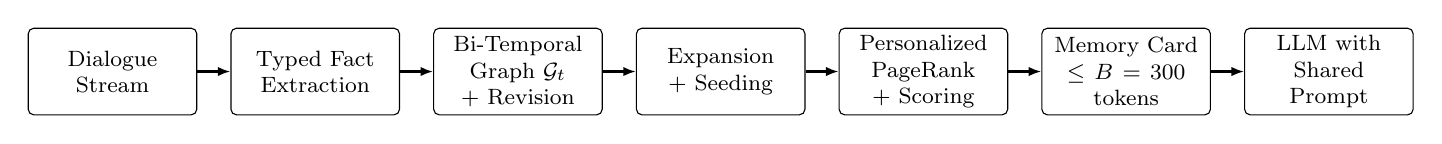
\begin{tikzpicture}[
  blk/.style={draw, rounded corners=2pt, align=center, font=\footnotesize,
              text width=2.0cm, minimum height=1.1cm, inner sep=2pt},
  arr/.style={-{Latex[length=1.6mm]}, thick},
  node distance=0.42cm]
\node[blk] (d) {Dialogue\\Stream};
\node[blk, right=of d] (x) {Typed Fact\\Extraction};
\node[blk, right=of x] (g) {Bi-Temporal\\Graph $\mathcal{G}_t$\\+ Revision};
\node[blk, right=of g] (h) {Expansion\\+ Seeding};
\node[blk, right=of h] (p) {Personalized\\PageRank\\+ Scoring};
\node[blk, right=of p] (s) {Memory Card\\$\le B=300$\\tokens};
\node[blk, right=of s] (l) {LLM with\\Shared\\Prompt};
\foreach \a/\b in {d/x,x/g,g/h,h/p,p/s,s/l} \draw[arr] (\a) -- (\b);
\end{tikzpicture}
\caption{ESD-Lite pipeline. Each user message is turned into typed, dated facts that update a bi-temporal knowledge graph without deleting anything. At question time, the question is expanded into the concepts it implies, graph nodes are seeded and scored with Personalized PageRank, and the best facts are packed into a Memory Card of at most 300 tokens that is sent to the LLM.}
\label{fig_arch}
\end{figure*}

ESD-Lite has six stages (Fig.~\ref{fig_arch}). Stages A--C run when a message arrives; stages D--F run when a question arrives.

\subsection{Typed Fact Extraction}
After each user message, the LLM fills a fixed schema through structured output. Each extracted fact has a \emph{kind} in \{\code{constraint}, \code{decision}, \code{event}, \code{fact}\}; a short third-person \emph{statement}; a \emph{slot}, a stable topic key such as \code{user.home\_city} that the extractor is asked to reuse from the list of existing slots; the \emph{entities} it mentions; and a \emph{valid-from} date. For constraints and decisions the extractor also lists 6--10 \emph{triggers}: situations in which the fact will matter later, including non-obvious ones (a nut allergy yields triggers such as \emph{desserts}, \emph{baked goods} and \emph{trail mix}). The prompt requires faithfulness (a dislike must not become an allergy). Relative dates (``this week'', ``last month'') are resolved against anchor dates computed in code (yesterday, the Monday of this and last week, the first day of this and last month), which removes date arithmetic from the model.

\subsection{Bi-Temporal Knowledge Graph}
Memory is a directed multigraph $\mathcal{G}_t = (\mathcal{V}_F \cup \mathcal{V}_E,\ \mathcal{E}_{\text{ABOUT}} \cup \mathcal{E}_{\text{SUP}})$ of fact nodes $\mathcal{V}_F$ and entity nodes $\mathcal{V}_E$. Each fact $f$ is linked to its entities by ABOUT edges and carries a bi-temporal stamp \cite{b_temporaldb,b_zep}
\begin{equation}
T(f) = \big\langle [t_v^s, t_v^e),\ [t_x^s, t_x^e) \big\rangle,
\end{equation}
where $[t_v^s, t_v^e)$ is the valid time (when the fact holds in the user's life) and $[t_x^s, t_x^e)$ the transaction time (when the system learned it and when it stopped believing it). A fact is \emph{active} while it has not been superseded.

\subsection{Non-Destructive Belief Revision}
For a new fact $f$, the candidate set is
\begin{equation}
\begin{split}
\mathcal{K}(f) = \{g : \text{slot}(g) = \text{slot}(f)\}\ \cup\ &\operatorname{Top}_4\{g : \cos(\mathbf{e}(f), \mathbf{e}(g)) \\
 &\qquad \ge 0.6\},
\end{split}
\end{equation}
taken over active facts. For each candidate the LLM first writes a one-sentence comparison and then labels the pair \code{same}, \code{replaces} or \code{unrelated}; asking for the rationale before the label corrected the errors we observed with label-only judging. A \code{same} label increments the mention count of the existing fact. A \code{replaces} label adds $f$ and revises the old fact $g$ as
\begin{align}
t_v^e(g) &\leftarrow t_v^s(f) \quad (\text{or } t_{\text{now}} \text{ if } t_v^s(f) < t_v^s(g)),\\
t_x^e(g) &\leftarrow t_{\text{now}}, \qquad \mathcal{E}_{\text{SUP}} \leftarrow \mathcal{E}_{\text{SUP}} \cup \{(f, g)\}.
\end{align}
Nothing is deleted: superseded facts remain queryable, which lets the system answer questions about the past and makes revision errors recoverable.

\subsection{Retrieval: Expansion, Seeding and Link Following}
\textit{Implication expansion.} The LLM lists 6--10 concepts implied by the question $q$ (for a macaron recipe: almond flour, egg whites, baking, and so on), giving the query set $\mathcal{Q} = \{q\} \cup X(q)$. Facts are embedded as their statement together with their triggers, so a stored constraint can meet a request through either side.

\textit{Seeding.} For every active fact and entity $n$, and for the current version of every superseded fact, we compute
\begin{equation}
s(n) = \max_{x \in \mathcal{Q}} \cos\big(\mathbf{e}(x), \mathbf{e}(n)\big), \qquad s_q(n) = \cos\big(\mathbf{e}(q), \mathbf{e}(n)\big).
\end{equation}
Up to 10 seeds are selected: 4 places are reserved for the best matches of the question itself (by $s_q$), and the rest are filled by $s$, with threshold $\theta = 0.20$. The reservation prevents vague expansion concepts from crowding out direct matches. When a superseded fact matches, its current version is seeded, and its card line carries the history.

\textit{Personalized PageRank.} On the undirected fact--entity graph (with the hub entity ``user'' removed), we compute \cite{b_ppr,b_hipporag}
\begin{equation}
\boldsymbol{\pi} = \alpha \mathbf{P}^{\top} \boldsymbol{\pi} + (1 - \alpha)\, \mathbf{p}, \qquad \alpha = 0.85,
\end{equation}
where $\mathbf{P}$ is the transition matrix and $\mathbf{p}$ the normalized seed scores. This reaches facts that are two steps away, for example from ``sister'' through the entity \emph{Rina} to ``Rina dislikes chocolate''.

\textit{Scoring.} Mirroring ESD's decaying edge weight $w_e(t) = \sigma(\mathbf{w}_r^{\top}\mathbf{x}_e)\, e^{-\lambda_r (t - t_v^s)} \log(1 + f_{u,v})$, but with measured similarity in place of the learned term, each fact receives
\begin{equation}
\begin{split}
r(f) = \Big(s(f)\,\mathbf{1}[f \in S] + 0.5\,\tfrac{\pi(f)}{\max_g \pi(g)}\Big)\, &e^{-\lambda_{k(f)}\,\Delta(f)} \\
 &\cdot \log_2\!\big(1 + m(f)\big),
\end{split}
\end{equation}
where $S$ is the seed set, $\Delta(f)$ the days since $f$ was last mentioned, $m(f)$ its mention count, and $\lambda_{k}$ a per-kind decay rate (0 for constraints, 0.005 per day for decisions, 0.01 for facts and events). All active constraints are always candidates; other facts are kept if they are seeds or have normalized PageRank of at least 0.05, up to the 12 best.

\subsection{Memory Card Under a Fixed Budget}
Candidates are ordered by $r(f)$, with constraints first, and added greedily to a card with four sections (rules, decisions, facts, events); a line is added only if the rendered card stays within $B = 300$ tokens. Each line carries its dates, and a fact with predecessors carries them inline, for example ``User moved from Chittagong to Dhaka (2025-02-24); replaced: `User lives in Chittagong' (2025-02-17 to 2025-02-24)''. The card is the textual counterpart of ESD's fixed budget of $K$ soft prefix tokens: its size does not depend on the length of the conversation.

\subsection{Answer Generation}
The LLM receives a system prompt with the date and weekday, the Memory Card, the last $w = 4$ messages of the current chat and the question. The system prompt is shared verbatim by every method we compare; it asks the model to respect the user's rules, check each suggested item against them, and prefer the most recent information.

\subsection{Relation to Full ESD}
Table~\ref{tab_mapping} maps each ESD component to its ESD-Lite counterpart. The symbolic half of ESD is implemented as designed; the neural half is replaced by retrieval and a text card, and is described as future work in Section~\ref{sec_future}.

\begin{table}[t]
\caption{Full ESD design versus the implemented ESD-Lite.}
\centering
\footnotesize
\setlength{\tabcolsep}{3pt}
\begin{tabular}{@{}L{2.55cm}L{2.95cm}L{2.3cm}@{}}
\toprule
\textbf{ESD component} & \textbf{ESD-Lite} & \textbf{Reason} \\
\midrule
Async 8B extractor & gpt-4o-mini, after each reply & No local GPU \\
Bi-temporal graph, AGM & Implemented as designed & Core of the method \\
HT-GNN, Fourier time & PPR + similarity + decay & No training data or GPU \\
Perceiver, $K{=}64$ latents & Greedy fill to 300 tokens & Same fixed-size goal \\
Soft prefix injection & Text Memory Card & API accepts text only \\
vLLM prefix caching & None & Needs self-hosting \\
\bottomrule
\end{tabular}
\label{tab_mapping}
\end{table}

\section{Experimental Setup}

\subsection{Benchmark Construction}
Because the planted fact and the question that needs it must be controlled exactly, we built a synthetic benchmark. The scenarios, the background messages and the filler messages were written by the research team with the assistance of an AI coding assistant. The benchmark is therefore authored by the same team that built the system; we mitigate this with a held-out split but do not remove it (Section~\ref{sec_limits}).
\begin{itemize}
\item \textbf{Background life}: 40 messages from one fictional user over six weeks (6 January to 14 February 2025) covering work, colleagues, friends, a pet, hobbies, food and tools, including topical near-misses for the tests (banana bread, a favourite dessert, a standing desk). Every method reads it first, so memory is realistically populated (35--37 facts for ESD-Lite, about 80 triples for Graph RAG).
\item \textbf{Fillers}: 20 chit-chat messages. Six follow every cue and ten follow the last cue, so that no cue remains in the $w = 4$ recent-message window.
\item \textbf{Scenarios}: 14 scenarios, each with dated cue messages, a question asked weeks later, and a written pass/fail criterion. Eight \emph{development} scenarios were used while building the system; six \emph{held-out} scenarios were written after the retriever was finalized and never used for tuning. Table~\ref{tab_scenarios} lists them.
\end{itemize}

\begin{table}[t]
\caption{Benchmark scenarios (D: development, H: held-out).}
\centering
\footnotesize
\setlength{\tabcolsep}{3pt}
\begin{tabular}{@{}lL{1.55cm}L{5.2cm}@{}}
\toprule
\textbf{ID} & \textbf{Category} & \textbf{Cue $\rightarrow$ later question} \\
\midrule
D1 & hidden rule & nut allergy $\rightarrow$ macaron recipe \\
D2 & changed decision & PostgreSQL, then MongoDB $\rightarrow$ connection code \\
D3 & budget & \$500 laptop budget $\rightarrow$ three laptop options \\
D4 & timeline & Chittagong, then Dhaka $\rightarrow$ city in February \\
D5 & multi-hop & sister Rina; Rina hates chocolate $\rightarrow$ cake for sister \\
D6 & goal & no alcohol before a marathon $\rightarrow$ Friday night plan \\
D7 & changed rule & vegetarian, then eats fish $\rightarrow$ high-protein dinner \\
D8 & negative rule & no meetings before 10am $\rightarrow$ daily standup time \\
H1 & hidden rule & celiac disease $\rightarrow$ breakfast before a flight \\
H2 & changed decision & Flutter, then native Swift $\rightarrow$ login screen code \\
H3 & budget & 30 minutes of exercise a day $\rightarrow$ weekly plan \\
H4 & timeline & Corolla, then Civic $\rightarrow$ car in February \\
H5 & multi-hop & Arif organizes lunch; Arif is vegan $\rightarrow$ restaurant \\
H6 & negative rule & motion sickness on boats $\rightarrow$ 3-day beach trip \\
\bottomrule
\end{tabular}
\label{tab_scenarios}
\end{table}

\subsection{Compared Methods}
All five methods use gpt-4o-mini at temperature 0 for every generation step, the same answer prompt, and the same recent-message window.
\begin{itemize}
\item \textbf{No memory}: only the recent window.
\item \textbf{Full history}: every past message with its date.
\item \textbf{Vector RAG} \cite{b_rag}: each past message is a chunk embedded with text-embedding-3-small; the top 5 by cosine similarity are sent.
\item \textbf{Standard Graph RAG}: a local-search baseline in the style of LightRAG and GraphRAG \cite{b_lightrag,b_graphrag}. The LLM extracts triples from each message into an entity graph without dates or retirement; at question time it extracts keywords, which are matched to the top 5 entities (cosine $\ge 0.35$), and all triples one hop from them are sent as text, up to 2{,}000 tokens. Global community summarization is not implemented.
\item \textbf{ESD-Lite}: as in Section IV, with $B = 300$.
\end{itemize}

\subsection{Metrics}
An LLM examiner (gpt-4o-mini, temperature 0) \cite{b_judge} marks each answer against the scenario's written criterion and gives a one-sentence reason. We report the Constraint Consistency Score (CCS, the pass rate), prompt tokens sent per question, memory tokens (the memory block only), response time to the complete answer, and the Context Compression Ratio $\text{CCR} = 1 - |\mathcal{C}(q)| / |\mathcal{D}|$ in tokens. The examiner's marks were spot-checked by hand.

\subsection{Implementation}
ESD-Lite is written in Python with NetworkX for the graph and PageRank, an SQLite cache for embeddings, and the OpenAI API for all model calls. A Streamlit application places the chat next to the ESD-Lite graph and the Graph RAG graph, built from the same messages, and shows both answers to each question. The final evaluation run made 714 API calls and runs on a commodity laptop without a GPU.

\section{Results}

\subsection{Main Results}
Table~\ref{tab_main} shows the final run. ESD-Lite passed all 14 scenarios, including all 6 held-out scenarios. Full history and vector RAG each failed one scenario, standard Graph RAG failed five, and the no-memory baseline passed two by chance.

\begin{table}[t]
\caption{Final run: 14 scenarios, gpt-4o-mini, temperature 0.}
\centering
\footnotesize
\setlength{\tabcolsep}{2.6pt}
\begin{tabular}{@{}lcccccc@{}}
\toprule
\textbf{Method} & \textbf{Dev} & \textbf{Held} & \textbf{CCS} & \textbf{Prompt} & \textbf{Memory} & \textbf{Time} \\
 & (8) & (6) & (\%) & tokens & tokens & (s) \\
\midrule
No memory & 0 & 2 & 14.3 & 231 & 0 & 2.30 \\
Full history & 8 & 5 & 92.9 & 1{,}263 & 1{,}042 & 3.07 \\
Vector RAG & 7 & 6 & 92.9 & 331 & 105 & 3.20 \\
Std.\ Graph RAG & 4 & 5 & 64.3 & 275 & 51 & 4.03 \\
\midrule
\textbf{ESD-Lite} & \textbf{8} & \textbf{6} & \textbf{100.0} & 488 & 272 & 4.85 \\
\bottomrule
\end{tabular}
\label{tab_main}
\end{table}

\begin{table}[t]
\caption{Per-scenario outcomes of the final run (\cmark{} pass, \xmark{} fail).}
\centering
\footnotesize
\setlength{\tabcolsep}{4pt}
\begin{tabular}{@{}lccccc@{}}
\toprule
\textbf{ID} & \textbf{None} & \textbf{Full} & \textbf{Vector} & \textbf{Graph} & \textbf{ESD-Lite} \\
\midrule
D1 hidden rule & \xmark & \cmark & \xmark & \xmark & \cmark \\
D2 changed decision & \xmark & \cmark & \cmark & \xmark & \cmark \\
D3 budget & \xmark & \cmark & \cmark & \xmark & \cmark \\
D4 timeline & \xmark & \cmark & \cmark & \xmark & \cmark \\
D5 multi-hop & \xmark & \cmark & \cmark & \cmark & \cmark \\
D6 goal & \xmark & \cmark & \cmark & \cmark & \cmark \\
D7 changed rule & \xmark & \cmark & \cmark & \cmark & \cmark \\
D8 negative rule & \xmark & \cmark & \cmark & \cmark & \cmark \\
H1 hidden rule & \cmark & \cmark & \cmark & \cmark & \cmark \\
H2 changed decision & \xmark & \cmark & \cmark & \cmark & \cmark \\
H3 budget & \xmark & \cmark & \cmark & \cmark & \cmark \\
H4 timeline & \xmark & \cmark & \cmark & \xmark & \cmark \\
H5 multi-hop & \xmark & \cmark & \cmark & \cmark & \cmark \\
H6 negative rule & \cmark & \xmark & \cmark & \cmark & \cmark \\
\bottomrule
\end{tabular}
\label{tab_grid}
\end{table}

\textit{Hidden links.} In D1 the allergy shares no words with the macaron request. Vector RAG retrieved five food- and weekend-related messages (banana bread, a favourite dessert, biryani, a drink and a hobby) but not the allergy, and answered with an almond-flour recipe; Graph RAG did the same. ESD-Lite expanded the question to \emph{almond flour}, which matched the stored allergy rule and its triggers, and replaced the flour.

\textit{Changes and time.} Standard Graph RAG, which has no validity times, could not tell which city or car was current in February (D4, H4) and, after the database switch, still held both ``uses PostgreSQL'' and ``uses MongoDB''. ESD-Lite answered both temporal questions from the dated history on its card.

\textit{Full history.} Full history was as accurate as ESD-Lite on the development set, but in H6 it suggested banana-boat rides although the ``no boats'' rule was in its prompt, an instance of a rule being overlooked in a longer context.

\subsection{Qualitative Case Study}
We ran a fixed six-question demonstration protocol in the application, asking each question in a new chat two weeks after the facts were given. ESD-Lite passed all six; standard Graph RAG failed five. Its failures show how keyword-to-entity matching goes wrong (Table~\ref{tab_case}): ``daily standup'' matched the entity ``standing desk'', and ``20 February'' matched ``end of February''.

\begin{table}[t]
\caption{Demonstration protocol: ESD-Lite vs.\ standard Graph RAG, with the entities Graph RAG matched.}
\centering
\footnotesize
\setlength{\tabcolsep}{3pt}
\begin{tabular}{@{}L{1.75cm}L{1.45cm}L{1.35cm}L{3.0cm}@{}}
\toprule
\textbf{Question} & \textbf{ESD-Lite} & \textbf{Graph RAG} & \textbf{Graph RAG matched} \\
\midrule
Macaron recipe & \cmark{} nut-free & \xmark{} almond & baking banana bread, weekend \\
Standup time & \cmark{} 10:00 & \xmark{} 9:00 & standing desk, team \\
Laptop options & \cmark{} $\le$\$500 & \xmark{} $>$\$500 & 2019 ThinkPad, services \\
Friday night & \cmark{} no alcohol & \xmark{} bar & Wednesday evening, parents \\
City on 20 Feb. & \cmark{} Chittagong & \xmark{} unknown & end of February, 12 May \\
Database code & \cmark{} MongoDB & \cmark{} MongoDB & invoicing service, PostgreSQL \\
\bottomrule
\end{tabular}
\label{tab_case}
\end{table}

For the database question Graph RAG answered correctly in this run, but it failed in 7 of the 9 runs of that question across our experiments, writing PostgreSQL code or code for both databases.

\subsection{Cost}
ESD-Lite sent 488 prompt tokens per question on average, 61.4\% fewer than full history (1{,}263), with Memory Cards of 218 to 300 tokens and a CCR of 73.9\%. It sent more than vector RAG (331) and Graph RAG (275), which retrieve less but miss more. The advantage over full history grows with conversation length because the card is bounded while the history is not. Table~\ref{tab_growth} counts the tokens of the full history as the conversation grows, using the benchmark's own messages; the full history exceeds the entire card budget after about 25 messages.

\begin{table}[t]
\caption{Memory tokens sent per question as the conversation grows.}
\centering
\footnotesize
\setlength{\tabcolsep}{3.4pt}
\begin{tabular}{@{}lccccccc@{}}
\toprule
\textbf{Messages} & 10 & 25 & 50 & 100 & 200 & 400 & 800 \\
\midrule
Full history & 225 & 499 & 963 & 1{,}916 & 3{,}762 & 7{,}496 & 14{,}922 \\
ESD-Lite card & \multicolumn{7}{c}{at most 300 at every length} \\
\bottomrule
\end{tabular}
\label{tab_growth}
\end{table}

\textit{Latency.} ESD-Lite was the slowest method (4.85\,s versus 3.20\,s for vector RAG) because it makes one extra LLM call to expand the question and sends a larger memory block.

\subsection{Development History and Error Analysis}
Table~\ref{tab_runs} lists every evaluation run. Run~1 exposed that questions about the past failed because superseded facts were not searchable and vague expansion concepts crowded out direct matches; the history-aware seeding and the reserved question seeds fixed this. Preparing the demonstration exposed an incorrect resolution of ``this week'', which led to the code-computed date anchors used in run~4. The held-out scenarios were added after the retriever fix. Standard Graph RAG's score varied between runs (7 and 9 of 14) because its extracted triples differ from run to run.

\begin{table}[t]
\caption{All evaluation runs (passes out of the scenarios run).}
\centering
\footnotesize
\setlength{\tabcolsep}{3pt}
\begin{tabular}{@{}L{3.1cm}ccccc@{}}
\toprule
\textbf{Run (change before it)} & \textbf{ESD} & \textbf{Full} & \textbf{Vec.} & \textbf{Graph} & \textbf{None} \\
\midrule
1: first run (8 dev.) & 7/8 & 8/8 & 7/8 & 2/8 & 1/8 \\
2: history-aware seeding & 8/8 & 8/8 & 7/8 & 2/8 & 0/8$^{*}$ \\
3: held-out set added & 14/14 & 14/14 & 13/14 & 7/14 & 2/14 \\
4: date anchors (final) & 14/14 & 13/14 & 13/14 & 9/14 & 2/14 \\
\bottomrule
\end{tabular}
\\[2pt]
{\scriptsize $^{*}$After tightening one criterion that no-memory had passed by suggesting nothing.}
\label{tab_runs}
\end{table}

The hand check of the examiner found two lenient marks, both favouring the no-memory baseline: one criterion was tightened and the saved answers re-marked, and the other (a gluten-free breakfast that included granola) was left as marked. Memory writing is imperfect: in the evaluation's background memory, one of the 40 messages caused a wrong replacement (a new hobby replaced an older, still-valid one). Because nothing is deleted, the older fact still appeared on the card as history, and the error did not change any outcome.

\section{Limitations}\label{sec_limits}
This is a pilot study. (i) The benchmark has 14 scenarios, and ESD-Lite's lead over full history and vector RAG is one scenario each, so no claim of statistical significance is made. (ii) The benchmark is synthetic and was written by the team that built the system; the held-out split prevents tuning to those scenarios but does not make them independent. (iii) Histories are short (about 1{,}000 tokens), which favours full history; public benchmarks such as LoCoMo are an order of magnitude longer. (iv) One model family both answers and grades; the examiner was spot-checked but not validated against human raters. (v) ESD-Lite is slower than vector RAG and sends more tokens than the retrieval baselines. (vi) The neural components of ESD were not implemented, so none of ESD's claims about soft-prefix steering or constant prefill cost are tested here.

\section{Future Work}\label{sec_future}

\subsection{Neural Soft-Prefix Projection}
The main next step is the neural half of ESD on an open-weight model that accepts embedding inputs. Node features $\mathbf{x}_v$ from a frozen text encoder would be combined with continuous time encodings of the elapsed time $\Delta t = t - t_v^s$ \cite{b_tgat,b_tgn}:
\begin{equation}
\boldsymbol{\psi}(\Delta t) = \big[ \cos(\omega_1 \Delta t), \sin(\omega_1 \Delta t), \dots, \sin(\omega_{d_T/2} \Delta t) \big]^{\top}.
\end{equation}
A heterogeneous temporal GNN (HT-GNN) with relation-specific attention would update node states over $L_{\text{GNN}} = 3$ layers:
\begin{equation}
\begin{split}
\mathbf{h}_v^{(l+1)} = \mathbf{W}_O^{(l)} \sum_{r \in \mathcal{R}} \sum_{u \in \mathcal{N}_r(v)} \alpha_{uv}^r
 \Big( &\mathbf{W}_V^r \mathbf{h}_u^{(l)} \\
 &+ \mathbf{W}_T^r \boldsymbol{\psi}(t - t_e) \Big),
\end{split}
\end{equation}
with attention scores
\begin{equation}
s_{uv}^r = \text{LeakyReLU}\big(\mathbf{a}_r^{\top} [\mathbf{W}_Q^r \mathbf{h}_v \,\|\, \mathbf{W}_K^r \mathbf{h}_u \,\|\, \mathbf{W}_T^r \boldsymbol{\psi}(t - t_e)]\big)
\end{equation}
normalized with a softmax jointly over relations and neighbours to give $\alpha_{uv}^r$. A Perceiver Resampler \cite{b_perceiverio,b_flamingo} with $K = 64$ learnable latents $\mathbf{Z}$ would compress the node states $\mathbf{H}$ into a fixed prefix:
\begin{equation}
\mathbf{Z}' = \text{Softmax}\!\left(\frac{\mathbf{Z}\mathbf{W}_Q (\mathbf{H}\mathbf{W}_K)^{\top}}{\sqrt{d_k}}\right) \mathbf{H}\mathbf{W}_V + \mathbf{Z},
\end{equation}
\begin{equation}
\mathbf{P}_{\text{soft}} = \text{FFN}\big(\text{LayerNorm}(\mathbf{Z}')\big) + \mathbf{Z}' \in \mathbb{R}^{K \times d_{\text{LLM}}},
\end{equation}
which is prepended to the token embeddings, $\mathbf{E}_{\text{in}} = [\mathbf{P}_{\text{soft}} \,\|\, \mathbf{E}_{\text{tok}}(X)]$ \cite{b_prefix,b_gretriever}. Training would follow two stages: contrastive alignment of the pooled prefix with response embeddings using an InfoNCE loss \cite{b_infonce}, then next-token training with the LLM frozen and LoRA adapters \cite{b_lora}:
\begin{equation}
\mathcal{L}_{\text{LM}} = -\sum_{i=1}^{M} \log P\big(y_i \mid \mathbf{P}_{\text{soft}}, y_{<i}\big).
\end{equation}
ESD-Lite's Memory Cards and examiner verdicts could supply training targets. The key comparison is soft prefix versus text card at an equal budget.

\subsection{Serving Efficiency}
With a self-hosted engine such as vLLM \cite{b_vllm}, the prefix could be bound to reserved placeholder tokens and its KV blocks reused while the graph is unchanged, indexed by a hash of the active subgraph. This would test ESD's claim of constant prefill cost, which a hosted text API cannot test.

\subsection{Stronger Evaluation}
We plan to (i) evaluate on public benchmarks, namely LoCoMo \cite{b_locomo}, LongMemEval \cite{b_longmemeval} and Multi-Session Chat \cite{b_msc}, and compare directly with HippoRAG~2 \cite{b_hipporag2} and Zep \cite{b_zep}; (ii) collect held-out scenarios written by people who have not seen the system; (iii) validate the examiner against human raters and a stronger judge model; (iv) report variance over repeated runs; and (v) run ablations that remove trigger anticipation, implication expansion, revision, history-aware seeding and the reserved question seeds, and vary the card budget $B$.

\subsection{System Improvements}
Extraction should run asynchronously, as in the full ESD design, once ordering guarantees are in place. The hand-set decay rates and weights in $r(f)$ could be learned. Latency could be reduced by running expansion in parallel with embedding and by caching expansions. Scaling to tens of thousands of facts will require a graph database, an approximate nearest-neighbour index and ranking among constraints. A user-facing way to inspect and correct memory would make revision errors fixable by the user.

\section{Conclusion}
We presented ESD-Lite, a hosted-API instantiation of Episodic Schema Distillation that stores conversational memory as a typed, bi-temporal knowledge graph with non-destructive revision, finds hidden links through trigger anticipation, implication expansion and link following, and sends a Memory Card of bounded size. In a controlled pilot on 14 scenarios, it respected the remembered constraint in every scenario, matched or exceeded full history, vector RAG and a standard Graph RAG baseline, and sent 61\% fewer prompt tokens than full history, at the cost of higher latency than retrieval baselines. These results are preliminary; the neural soft-prefix projection and evaluation on public benchmarks are the next steps.

\section*{Acknowledgment}
Parts of the implementation, the evaluation scenarios and the text of this paper were drafted with the assistance of an AI coding assistant (Claude, Anthropic). The authors reviewed all content and take responsibility for it.

\begin{thebibliography}{00}
\bibitem{b_locomo} A. Maharana, D.-H. Lee, S. Tulyakov, M. Bansal, F. Barbieri, and Y. Fang, ``Evaluating very long-term conversational memory of LLM agents,'' \textit{arXiv preprint arXiv:2402.17753}, 2024.
\bibitem{b_msc} J. Xu, A. Szlam, and J. Weston, ``Beyond goldfish memory: Long-term open-domain conversation,'' in \textit{Proc. ACL}, 2022.
\bibitem{b_longmemeval} D. Wu, H. Wang, W. Yu, Y. Zhang, K.-W. Chang, and D. Yu, ``LongMemEval: Benchmarking chat assistants on long-term interactive memory,'' in \textit{Proc. Int. Conf. Learn. Representations (ICLR)}, 2025.
\bibitem{b_lostmiddle} N. F. Liu, K. Lin, J. Hewitt, A. Paranjape, M. Bevilacqua, F. Petroni, and P. Liang, ``Lost in the middle: How language models use long contexts,'' \textit{Trans. Assoc. Comput. Linguistics}, vol. 12, 2024.
\bibitem{b_memgpt} C. Packer, S. Wooders, K. Lin, V. Fang, S. G. Patil, I. Stoica, and J. E. Gonzalez, ``MemGPT: Towards LLMs as operating systems,'' \textit{arXiv preprint arXiv:2310.08560}, 2023.
\bibitem{b_streaming} G. Xiao, Y. Tian, B. Chen, S. Han, and M. Lewis, ``Efficient streaming language models with attention sinks,'' in \textit{Proc. Int. Conf. Learn. Representations (ICLR)}, 2024.
\bibitem{b_h2o} Z. Zhang, Y. Sheng, T. Zhou, T. Chen, L. Zheng, R. Cai, Z. Song, Y. Tian, C. R{\'e}, C. Barrett, Z. Wang, and B. Chen, ``H$_2$O: Heavy-hitter oracle for efficient generative inference of large language models,'' in \textit{Proc. Adv. Neural Inf. Process. Syst. (NeurIPS)}, 2023.
\bibitem{b_rag} P. Lewis, E. Perez, A. Piktus, F. Petroni, V. Karpukhin, N. Goyal, H. K{\"u}ttler, M. Lewis, W. Yih, T. Rockt{\"a}schel, S. Riedel, and D. Kiela, ``Retrieval-augmented generation for knowledge-intensive NLP tasks,'' in \textit{Proc. Adv. Neural Inf. Process. Syst. (NeurIPS)}, 2020.
\bibitem{b_graphrag} D. Edge, H. Trinh, N. Cheng, J. Bradley, A. Chao, A. Mody, S. Truitt, and J. Larson, ``From local to global: A graph RAG approach to query-focused summarization,'' \textit{arXiv preprint arXiv:2404.16130}, 2024.
\bibitem{b_lightrag} Z. Guo, L. Xia, Y. Yu, T. Ao, and C. Huang, ``LightRAG: Simple and fast retrieval-augmented generation,'' \textit{arXiv preprint arXiv:2410.05779}, 2024.
\bibitem{b_hipporag} B. J. Guti{\'e}rrez, Y. Shu, Y. Gu, M. Yasunaga, and Y. Su, ``HippoRAG: Neurobiologically inspired long-term memory for large language models,'' in \textit{Proc. Adv. Neural Inf. Process. Syst. (NeurIPS)}, 2024.
\bibitem{b_hipporag2} B. J. Guti{\'e}rrez et al., ``From RAG to memory: Non-parametric continual learning for large language models,'' in \textit{Proc. Int. Conf. Mach. Learn. (ICML)}, 2025.
\bibitem{b_zep} P. Rasmussen et al., ``Zep: A temporal knowledge graph architecture for agent memory,'' \textit{arXiv preprint arXiv:2501.13956}, 2025.
\bibitem{b_temporaldb} R. Snodgrass and I. Ahn, ``Temporal databases,'' \textit{Computer}, vol. 19, no. 9, pp. 35--42, 1986.
\bibitem{b_agm} C. E. Alchourr{\'o}n, P. G{\"a}rdenfors, and D. Makinson, ``On the logic of theory change: Partial meet contraction and revision functions,'' \textit{J. Symbolic Logic}, vol. 50, no. 2, pp. 510--530, 1985.
\bibitem{b_ppr} T. H. Haveliwala, ``Topic-sensitive PageRank,'' in \textit{Proc. Int. World Wide Web Conf. (WWW)}, 2002.
\bibitem{b_judge} L. Zheng, W.-L. Chiang, Y. Sheng, S. Zhuang, Z. Wu, Y. Zhuang, Z. Lin, Z. Li, D. Li, E. P. Xing, H. Zhang, J. E. Gonzalez, and I. Stoica, ``Judging LLM-as-a-judge with MT-Bench and Chatbot Arena,'' in \textit{Proc. Adv. Neural Inf. Process. Syst. (NeurIPS) Datasets and Benchmarks Track}, 2023.
\bibitem{b_prefix} X. L. Li and P. Liang, ``Prefix-tuning: Optimizing continuous prompts for generation,'' in \textit{Proc. ACL}, 2021, pp. 4582--4597.
\bibitem{b_perceiverio} A. Jaegle, S. Borgeaud, J.-B. Alayrac, et al., ``Perceiver IO: A general architecture for structured inputs \& outputs,'' in \textit{Proc. Int. Conf. Learn. Representations (ICLR)}, 2022.
\bibitem{b_flamingo} J.-B. Alayrac, J. Donahue, P. Luc, A. Miech, et al., ``Flamingo: A visual language model for few-shot learning,'' in \textit{Proc. Adv. Neural Inf. Process. Syst. (NeurIPS)}, 2022.
\bibitem{b_gretriever} X. He, Y. Tian, Y. Sun, N. V. Chawla, T. Laurent, Y. LeCun, X. Bresson, and B. Hooi, ``G-Retriever: Retrieval-augmented generation for textual graph understanding and question answering,'' in \textit{Proc. Adv. Neural Inf. Process. Syst. (NeurIPS)}, 2024.
\bibitem{b_tgat} D. Xu, C. Ruan, E. Korpeoglu, S. Kumar, and K. Achan, ``Inductive representation learning on temporal graphs,'' in \textit{Proc. Int. Conf. Learn. Representations (ICLR)}, 2020.
\bibitem{b_tgn} E. Rossi, B. Chamberlain, F. Frasca, D. Eynard, F. Monti, and M. Bronstein, ``Temporal graph networks for deep learning on dynamic graphs,'' \textit{arXiv preprint arXiv:2006.10637}, 2020.
\bibitem{b_infonce} A. van den Oord, Y. Li, and O. Vinyals, ``Representation learning with contrastive predictive coding,'' \textit{arXiv preprint arXiv:1807.03748}, 2018.
\bibitem{b_lora} E. J. Hu, Y. Shen, P. Wallis, Z. Allen-Zhu, Y. Li, S. Wang, L. Wang, and W. Chen, ``LoRA: Low-rank adaptation of large language models,'' in \textit{Proc. Int. Conf. Learn. Representations (ICLR)}, 2022.
\bibitem{b_vllm} W. Kwon, Z. Li, S. Zhuang, Y. Sheng, L. Zheng, C. H. Yu, J. E. Gonzalez, H. Zhang, and I. Stoica, ``Efficient memory management for large language model serving with PagedAttention,'' in \textit{Proc. ACM Symp. Operating Syst. Principles (SOSP)}, 2023.
\end{thebibliography}

\end{document}
